\documentclass[a4paper]{jpconf}
\usepackage{graphicx}
\usepackage{textcomp}

\begin{document}
\title{Systematic profiling to monitor and specify the software refactoring process of the LHCb experiment}

\author{Ben Couturier}
\address{CERN, CH-1211 Geneva 23, Switzerland}
\ead{ben.couturier@cern.ch}

\author{Emmanouil Kiagias}
\address{CERN, CH-1211 Geneva 23, Switzerland}
\ead{emmanouil.kiagias@cern.ch}

\author{Stefan B. Lohn}
\address{CERN, CH-1211 Geneva 23, Switzerland}
\ead{stefan.lohn@cern.ch}

\begin{abstract}
The LHCb collaboration develops and maintains large software frameworks, critical to the good performance of the experiments, that face challenges due to the increase of throughput requested from the physics side that will not be matched by the computing resources, and by new computing architectures such as many-core, that cannot be currently fully used due to the limited amount of memory available per core. In the coming years, a considerable refactoring effort will therefore be needed to vectorize and parallelize the code, to minimize hotspots and to reduce the impact of bottlenecks. It is crucial to guide the refactoring with a profiling system that gives hints to parts for possible and necessary source-code re-engineering and which kind of optimization could lead to final success.
\newline
Software optimization is a sophisticated process where all parts, compiler, operating system, libraries and chosen hardware play a role in. Intended improvements can have different effects on different platforms. To obtain precise information of the general performance, to make profiles comparable, reproducible and to verify the progress of performance in the framework, it is important to produce profiles more systematically in terms of regular profiling based on representative use cases and to perform regression tests. Once a general execution, monitoring and analysis platform is available, software metrics can be derived from the collected profiling results to trace changes in performance back and to create summary reports on a regular basis with an alert system if modifications led to significant performance degradations.
\end{abstract}

\section{Introduction}
\label{sec:introduction}

In large scale software solutions of high energy physics, performance is critical for efficient result extraction. Plenty of profiling tools are available and must be integrated to trace performance already from an early state in development. But often software is more evolving because of considerations of maintainability, usability, flexibility, due to necessary features implementation or urgent bug fixes, than due to performance optimization. Often it appears, that such information are not clearly and reliable available to determine the importance of performance optimizing measures. Hence, performance has less or no priority, also because there are no information about certain software behavior at all. The LHCb performance \& regression (PR) project tries to address this issue for the LHCb experiment at CERN to allow more intervention which relies on performance information.    
\newline
During its development phase, the LHCb software was constantly optimized; the profiling was however in responsibility of each developer, with no ``official'' profiling test suite defined and no record of the results. While this approach was effective in the framework development phase, there are no record of the evolution in software performance, nor of the current baseline. With a refactoring of the code under way it is therefore now necessary for LHCb to put systematic profiling tests in place, in order to ensure that there is no performance degradation.
\newline
This paper describes the LHCb PR framework, to profile the experiments software and to display results in a user friendly manner. This paper describes an overview about LHCb software and the objectives of the LHCb PR project in chapter \ref{sec:lhcb_computing}, the work-flow with some implementation aspects in chapter \ref{sec:workflow_and_implementation} and briefly goes into upcoming challenges in chapter \ref{sec:lhcbpr_and_beyond}.

\section{LHCb computing}
\label{sec:lhcb_computing}

\subsection{LHCb software}
\label{sec:lhcb_software}

The LHCb experiment software is based on Gaudi\cite{gaudi}, a C++ framework using generic and object-oriented features of C++ for computing intensive tasks, and python for configuring and structuring modules (algorithms, tools...). The application manager executes consecutive an abstract series of algorithms to process data objects from the transient store on request. Gaudi is providing core services and tools for applications to hide complexity and make future development and changes more transparent for users. It is a large-scale framework and is additionally used by ATLAS, Glast, Harp and other experiments.
\newline
Applications build on top of Gaudi are Moore, Brunel, DaVinci, Gauss, Boole and others. Moore is the implementation of the High-Level Trigger (HLT) to decide weather event data will be stored or not, Brunel is responsible for the offline reconstruction of tracks, DaVinci is the physics analysis framework, Gauss to simulate the particle transport and interaction through several detector modules, and Boole performs the digitization.

\subsection{Computing environment}
\label{sec:computing_environment}

The LHCb computing environment persists out of the computing resources accessed in the Worldwide LHC Computing Grid (WLCG), in Cloud Infrastructure and in the HLT farm located at the experiment. Additional, virtualization is used and just recently volunteer computing has been added. Some 100k CPU's are involved in the data processing. 
%35 GB/s of recorded data have to be processed by 1500 computing nodes of the Event Filtering Farm (EFF) of the HLT to be reduced to 70 MB/s \cite{lhcb_hlt_opt}.

\subsection{Integrated Profiling}
\label{sec:integrated_profiling}

In HEP computing it is a common method to measure performance via throughput (events processed per time unit). Thus the performance analysis is focused on the time linear and not the time constant part of processing. Instrumentation is an important advantage for profiling source-code in large scale frameworks like the applications from the LHCb experiment. Multiple profiling measures have been implemented in the Gaudi framework using the AuditorService \cite{status_gaudi} which provides an interface for executing code between events or algorithms processed.
\newline
Timing information from the operating system's process information are collected using the TimingAuditor and are printing a summary of time spend in the applications algorithms. Likewise information can be collected using the Memory- or MemStatAuditor for changes in memory as soon as they appear. Recent work \cite{intel_auditor} conducted by Mazurov and Couturier shows how to improve precision in profiling the event-loop using instrumentation routines of Intel's VTune\texttrademark Amplifier API, which can be added using the IntelAuditor. Another strategy is to collect information from the performance monitoring unit (PMU) of modern CPU architectures to collect information about hardware usage and issues such as cache-misses, branch-misprediction and more as done by Kruse and Kruzelecki \cite{modular_monitoring} for the Gaudi framework. Many of such kind of work has been performed to provide tools for developers to profile their code. Still, systematic usage or comparative profiling has been sparsely observed.

\subsection{Systematic Profiling}
\label{sec:integrated_profiling}

Three important aspects must be considered as crucial for systematic profiling. Profiles must become \textit{comparable}, \textit{reproducible} and \textit{representative} to allow regression analysis and to trace back changes in performance to source-code locations. For a series of regular profiles for several platforms, profiling must be limited to a small number of default cases and a fixed set of reference data. Reference data are also important to avoid variance due to different types of physics. This way differences in execution behavior between two revisions can be examined and traced back on changes in related source-code. On the other side, changing the reference set of physics events could later on be used to evaluate the needs of computing resources for upcoming data-taking periods and changing recorded event information.
%Systematic profiling should not only trace back hotspots and drawbacks of changes in code, but shell help to obtain and understanding which techniques, tool for optimization, or changing platforms are having a higher impact on saving computing resources.
\newline
Furthermore, profiles must be reproducible to be able to compare the test configuration of executed test jobs. This affects the job configuration, to log the software/platform information, as well as the run configuration provided by option files for Gaudi applications. Finally, gathered information should be precise and reliable making a regular execution of a series of test jobs necessary.
\newline
Hence the LHCb PR project has the following requirements.
\begin{enumerate}
 \item The expected huge amount of information must be centrally collected and easily become accessible. This can be achieved by using a web application as interface to support brief analysis of collected data.
 \item Profiling is a changing subject with new interesting technologies. A solution must be flexible to include new profiling tools. Information must be collected by parsing generated reports and hooking them onto a central database.
 \item To reduce work generic ways of navigation and visualization have to be investigated by trying to use supporting tools as much as available.
 \item Regular execution would be labor intensive without an automated execution chain. Automated triggering, setup and data collection of the profiling procedure simplifies systematic profiling attempts.
\end{enumerate}
To fulfill the objectives and requirements, the LHCb PR project contains three important technical aspects. First, the PRConfig project was created to store the run configuration in a version control system and to collect further job information and final profiling results into a central SQL database. Second, Jenkins \cite{jenkins} a continuous integration system is used to configure, trigger and submit test jobs and finally Django \cite{django} to support the web application to quickly visualize and propagate results. 

\begin{figure}
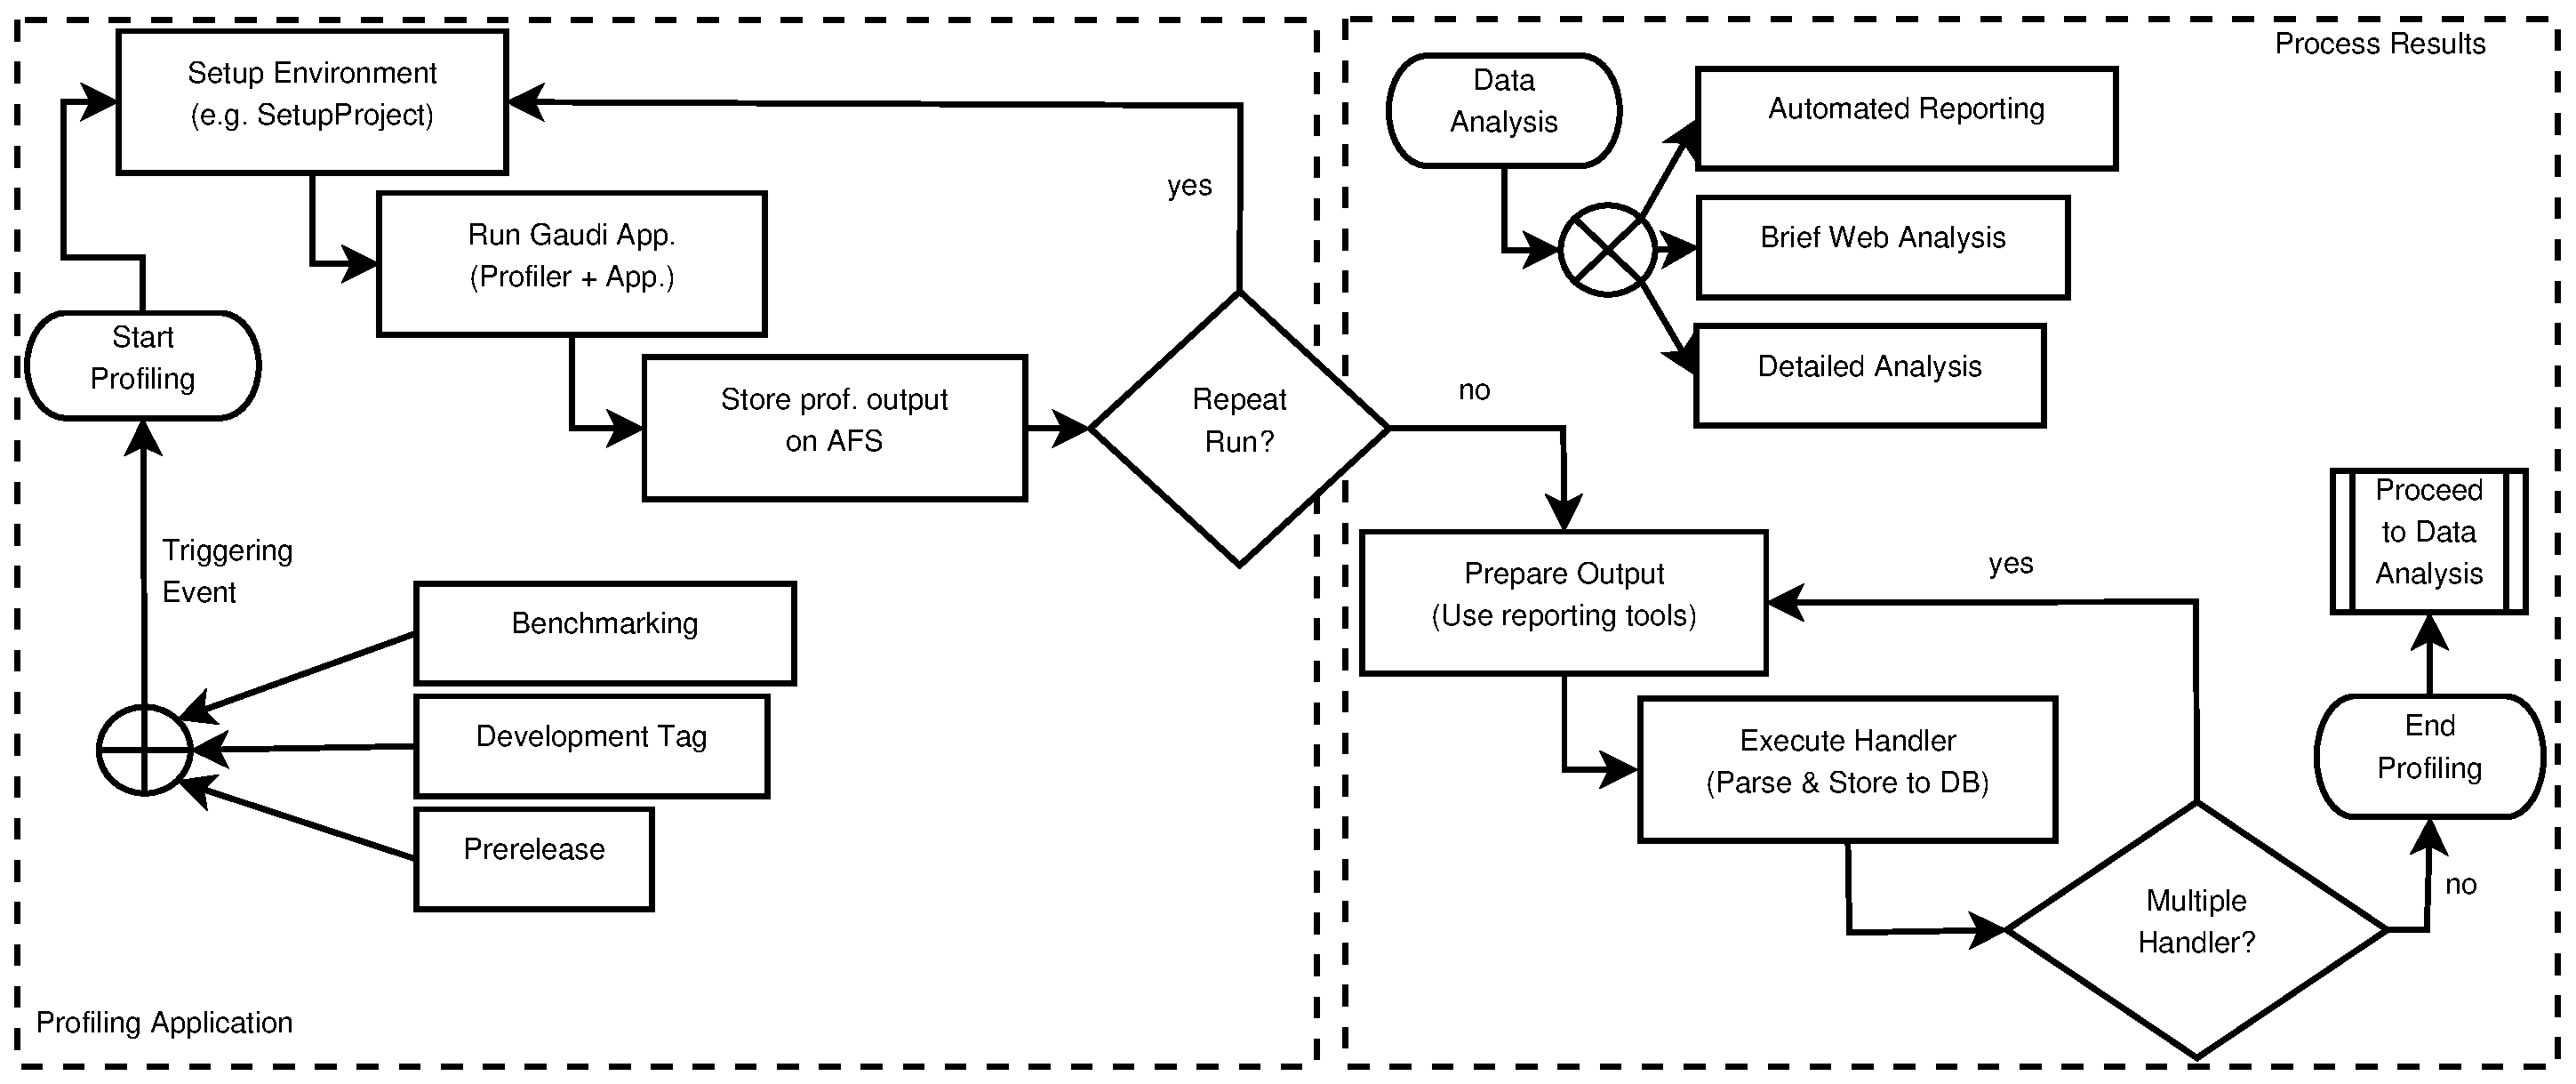
\includegraphics[width=\textwidth, height=5.6cm]{figures/profiling_process.eps}
\caption{\small \textit{The work-flow has three main parts. A) the test definition, triggering and job submission. B) the rob execution, repetition and data collection using data handlers. C) quick access to profiling results.}}
\label{fig:profiling_process}
\end{figure}

\section{LHCb PR project}
\label{sec:lhcbpr}

\subsection{Work-flow}
\label{sec:workflow}

The LHCb PR project provides support to conduct systematic profiling. The work-flow can technically be divided into three major parts, as in \mbox{figure \ref{fig:profiling_process}}, where Jenkins is used to configure, trigger and schedule test jobs before profiling (A). Before execution (B), a wrapper is downloaded and executed to hide the profiler specific setup. While execution, profiler information is gathered, profiles and log-files are stored on a distributed file system (AFS) for later detailed analysis. In the end, data handlers to parse reports and collect results are called, which are defined for distinct types of profiles and can provide additional job information like a comment, a profile class or a AFS path per job. Depending on the desired information, profiles can be filtered or combined with other available information in the data handler. Then, results are hooked onto a SQL database. In the end (C), the LHCb PR web analysis interface facilitates profile comparisons and helps detecting anomalies in performance.

\subsection{LHCb PR web interface}
\label{sec:lhcbpr_web_interface}

The core of the LHCb PR framework is a web interface based on Django to analyze profiles. The backbone of Django is using python to speed up development while keeping a certain amount of flexibility due to a variety of auxiliary modules available. Additionally, processing intensive tasks can be performed on the server-side while keeping the interface quick and smart.
\newline
The front-end can ruffly be divided into two main aspects, navigation and visualization. To navigate easily through data, results can directly accessed by their \textit{category}, a tuples of job description id, platform and host. To select categories, a generic selection menu allows to specify categories for comparison.  The generic menu is supplemented by a customized part, to specify profiling groups (different profiling information), attributes or filtering options, which are important to the specific visualization. Data access is also available on job level via a job table accessible through a table of different categories.
\newline
The current visualization supports what is called a top-down analysis. Different analysis types are referring to different ways of visualization in which data \textit{attributes}, a generic items for performance information, are shown. Attributes can be runtime, resident memory, possibly lost memory or more complex metrics. The Trend-Analysis, that figures out the progress of attributes cross versions or revisions, has been added to observe changes in the general performance during the code evolution. Significant changes become immediately conspicuous, but requires single attributes, e.g. one of many algorithms, to be tracked. The Overview-Analysis is about to show several attributes between two versions, platforms or configurations. Both, Trend and Overview, show entries with their statistical variance. To get more precise information about the distribution of attributes around their average the Basic-Analysis can be used.
\newline
Visualization is realized by ROOT histograms, where the python interface pyRoot simplifies the access to or by Google Charts that has demonstrated to be flexible and quick for implementation. The Basic-analysis is using ROOT histograms with the attributes dimension as x-axis and normalized about the amount of entries on the y-axis, e.g. see \mbox{figure \ref{fig:brunel_basic_libm}}. 

\subsection{Job distribution and triggering}
\label{sec:job_distribution}

To facilitate \textit{regular profiling} in a \textit{series of equal tests} to permit statistic evaluations, Jenkins helps to manage the job distribution to test hosts. The Test configurations, the composition of the job and the run configuration, can be prepared by creating generic parametrized jobs. Preprocessing, e.g. compiling packages with specific compiler flags or using different revisions of packages within specific a version, can be added. Jenkins organizes the inclusion of further hosts and it prevents interferences between multiple jobs running on the same machine by limiting job slots.
\newline
A cron-jobs like plugin in Jenkins can be used to induce a regular triggering event within the release- or build cycle. This way, from triggering to execution and data collection, no human intervention is necessary, what simplifies data collection and opens the way to point out reliable and significant changes in the software profile.

\subsection{Data collection}
\label{sec:data_collection}

Data collection is performed by \textit{data handlers} or bigger profiles are stored onto AFS. There are two different kinds of handlers to store data. First one can segregate information from reports to store results onto a database, and second, files which contain performance information can become available for downloading on the web-interface. To maintain flexibility for different profilers, the post-processing of a profiling job must prepare parsable reports. The LHCb PR Handler project hosts the various parsers to collect these data.

\begin{figure}[t]
\begin{minipage}[t]{0.3\textwidth}
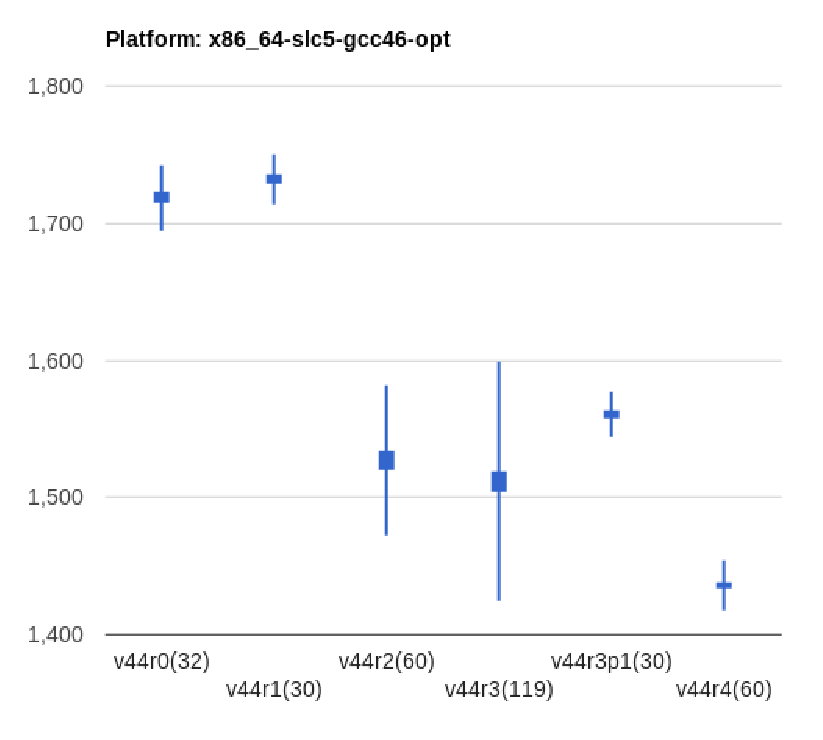
\includegraphics[scale=0.33]{figures/brunel_trend_analysis.eps}
\caption{\small \textit{Trend analysis (runtime [ms] \texttimes versions) of Brunel to monitor changes of specific attributes cross versions to observe the general performance.}}
\label{fig:brunel_trend}
\end{minipage}\hspace{1pc}
\begin{minipage}[t]{0.3\textwidth}
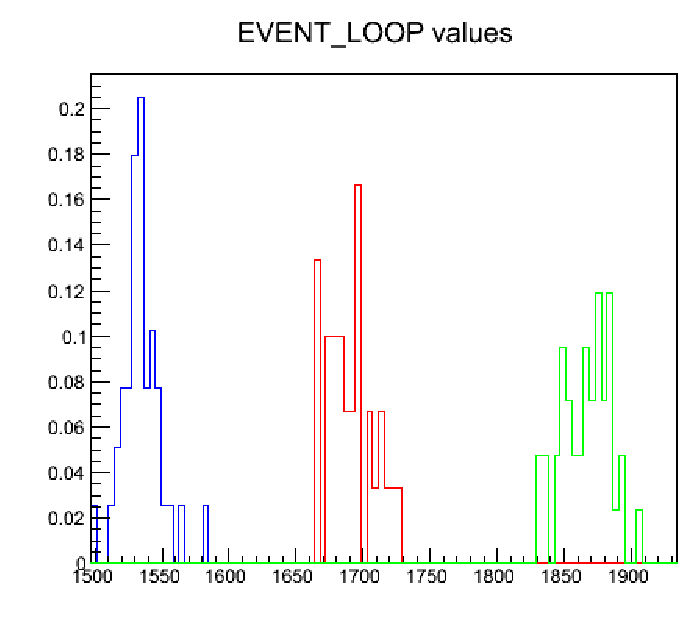
\includegraphics[scale=0.40]{figures/brunel_basic_libm.eps}
\caption{\small \textit{Shows runtime distribution ([ms] per event) using different math libraries. (blue) Intel, (red) elder libm, (green) updated libm of a new glibc version.}}
\label{fig:brunel_basic_libm}
\end{minipage}\hspace{1pc}
\begin{minipage}[t]{0.35\textwidth}
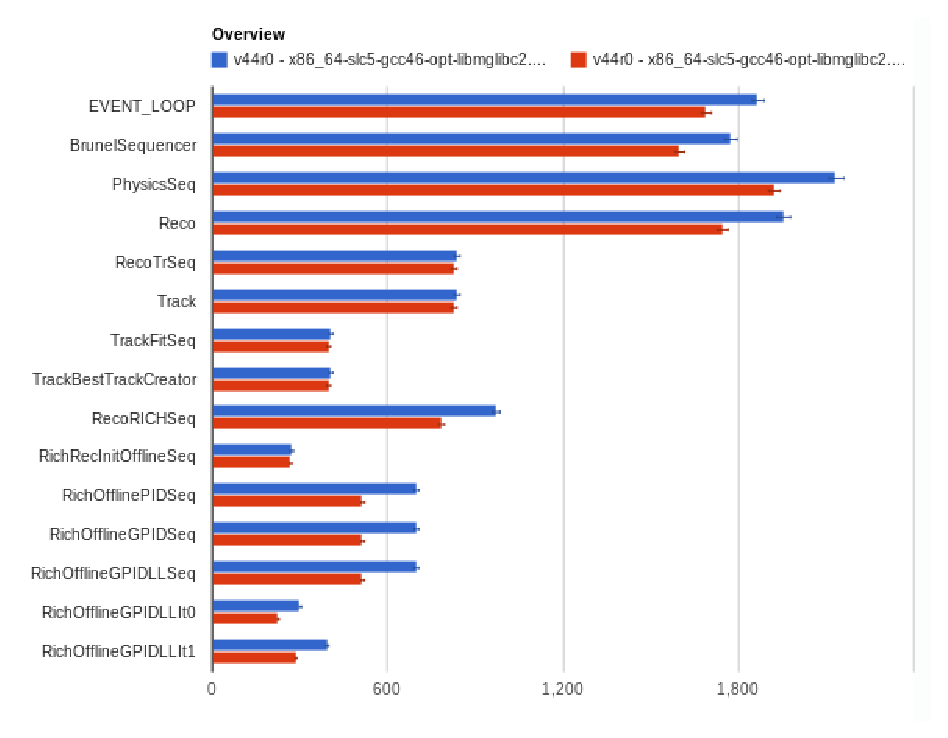
\includegraphics[width=1\textwidth, height=4cm]{figures/brunel_overview_analysis.eps}
\caption{\small \textit{Overview analysis of Brunel to get a fast impression of attributes behavior to others and cross versions, platform or differing configurations (options).}}
\label{fig:brunel_overview}
\end{minipage}
\end{figure}

\subsection{Test cases}
\label{sec:test_cases}

\textit{Use cases} are important to trace performance changes back to the evolving algorithms. \textit{Test cases} shell base on default use cases for best approximations to the production usage. Still, the sophisticated computing environments can influence runs on a non-predictive non-deterministic way, which hampers conclusions from regression analysis. Currently, the highest priority is to find software related issues, that can be addressed or have to be taken into account for upcoming decisions in resource allocation.
\newline
A few default cases for Brunel have been quickly evaluated, defined and are running now on a regular basis after each successful build. LHCb PR has demonstrated its importance already by observing simple timing information obtained by the TimingAuditor. Significant changes become immediately clear by observing the trend information cross versions as shown exemplary in \mbox{figure \ref{fig:brunel_trend}}. After observing performance degradation, further tests can be defined to use more precise profilers, like the IntelAuditor, for more details. One real example shows the changes found in the external math library, as shown in Figure \ref{fig:brunel_basic_libm}. Such information is important to be available before a release is done. % To get regular information on time spend in all libraries, VTune\texttrademark can be used for regular runs.
\newline
Unfortunately, the HLT framework Moore can not simply be reduced to a view common default cases, what makes it more difficult to trace back performance issues using a top-down analysis. The further complications are:
\begin{enumerate}
 \item The computing environment at the HLT farms are highly sophisticated with processes cloned to run multiple of them on a node and with events coming from the BufferManager.
 \item Single or a few default cases, as required, are not available because of constantly changing trigger configuration keys (TCKs), which define the algorithms involved.
\end{enumerate}
The first problem can only be addressed if users agree to a representative standard configuration. Since this is currently not available, no enhancements can here be made. The second problem can partially be addressed by not only splitting use cases, but also the software into parts for further investigations. This also simplifies tracing back performance issues to source-code locations and to help particular software development efforts. Finally the Overview-Analysis was adapted to be able to compare different run configurations, different option files with the same application and version.

\section{LHCb PR and beyond}
\label{sec:lhcbpr_and_beyond}

\subsection{Profiling accuracy}
\label{sec:profiling accuracy}

In the current state, the web-interface does not provide a resolution beyond algorithm level. More detailed information are only accessible via the collected profile information. The resolution of the web-interface is limited for two good reasons. First, developer shell be provided with profiles, but competing with the variety of visualization tools of highly sophisticated profilers is not feasible and second, systematic profiling must not completely replacing the local- and temporary profiling of single developers, since limited use cases will always hide information about performance of algorithms made for spare situations, and since performance changes can be compensated within a top-down view on the account of a single smallest unit, here an algorithm.
\newline
Another reason to limit the amount of performance data is, because of the already massive amount of collected data for regression analysis and hence, the expected amount of data for a series of runs with the same test configuration. Visualizing the regression analysis allows more precise information than a single run permits. But more precision leads to problems with unpredictable side effects of recent hardware features. They can influence runtime, e.g. by using frequency scaling or automated over-clocking. On the one side, these aspects can now precisely be analyzed, but needs on the other side also to be neutralized during regular profiling to detect software performance anomalies.

\subsection{Complementary information}
\label{sec:complementary_information}

Still it could be reasonable to increase the resolution to function level. A call stack of functions and runtime spent, would enable us to see if algorithm were calling objects first and executing lazy initialization. In particular for Gaudi, which allows a flexible order in which algorithms are called, it would be a . For instance tracking in the vertex detector is started by the first algorithm which requests these information and later on data can directly be accessed. This makes algorithm vary in their profile, what can currently not be reasonable traced back from the web analysis.
\newline
Due to the issue of the latter paragraph, the unordered execution of algorithms need to be addressed. This can be done by adding further complementary information, like a function call-stack for each algorithm to give a much higher resolution for finding anomalies in profiles than currently available, and it would make profiles of algorithms more comprehensive.
\newline
Another upcoming task is that if once a test case is fully implemented to be analyzed by several profilers in distinct runs, and if much more general information are available, these information could also be used to be correlated to each other. This way it would be possible to find the impact of design decisions and to validate existing methods or new concepts. Then open questions could be answered as knowledge base for further developments.
\newline
At the moment measurements like CPI, cache-misses, branch-misprediction and others are often mentioned, but can barely be correlated to real performance influences. Questions like how much exactly the call-stack depth influences runtime by occurring more cache-misses, and how does this influences current R\&D project like Gaudi-Hive by sharing cache among threads could then be emphasized by concrete numbers.

% \begin{figure}[t]
% \begin{minipage}[b]{0.33\textwidth}
% 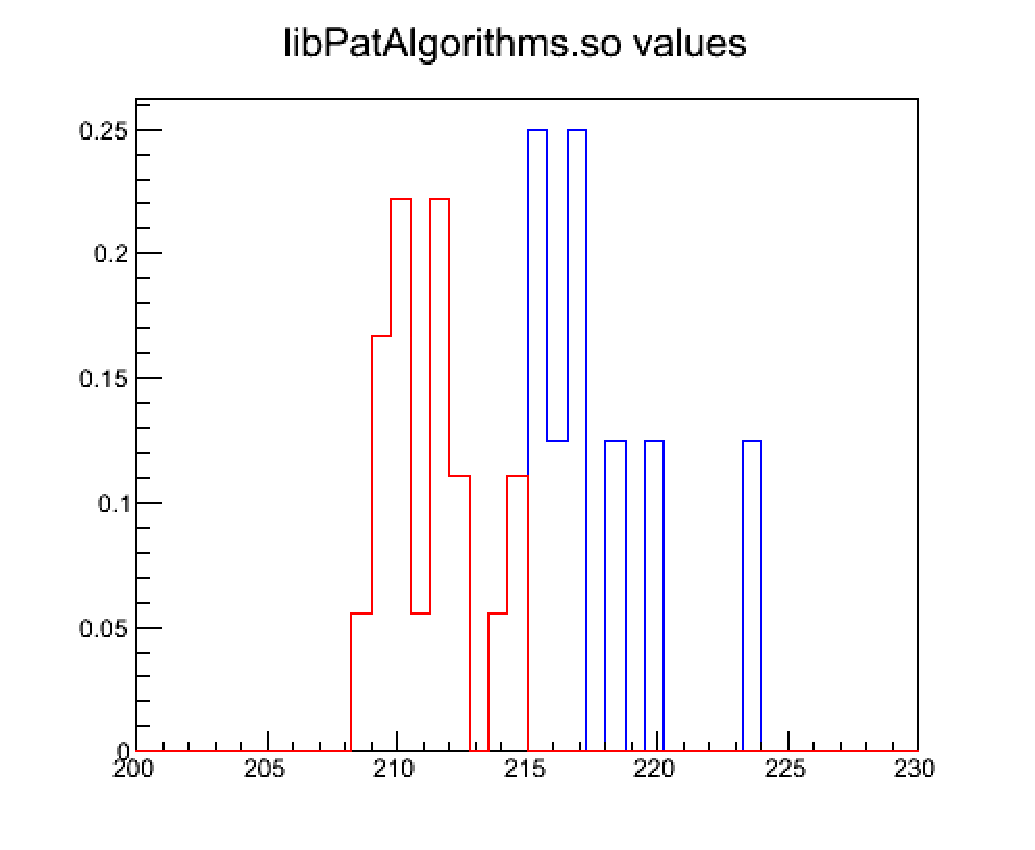
\includegraphics[scale=0.3]{figures/moore_basic_vect.eps}
% \caption{\small \textit{Comparing auto-vectorized library in Moore again unvectorized version.}}
% \label{fig:moore_basic}
% \end{minipage}\hspace{0.5cm}%
% \begin{minipage}[b]{0.60\textwidth}
% \centering
% 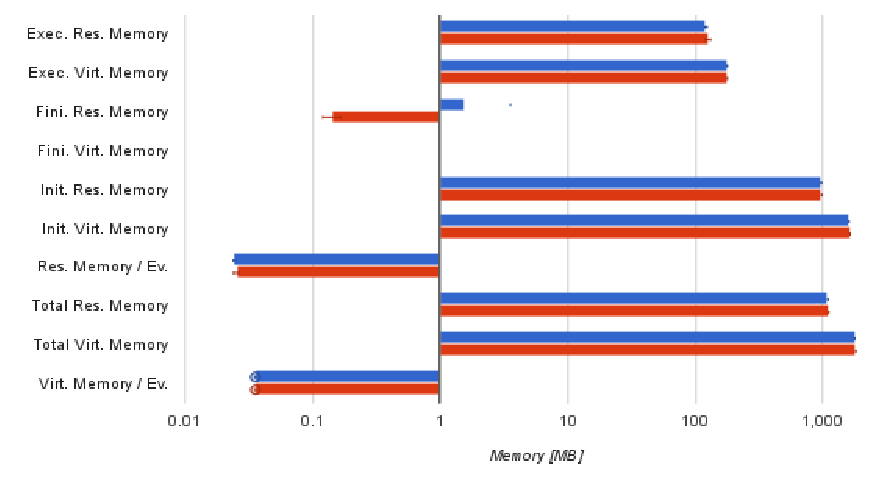
\includegraphics[scale=0.50]{figures/moore_overview_memory.eps}
% \caption{\small \textit{For some application memory consumption is crucial. An overview of several memory information to observe differences between version.}}
% \label{fig:moore_overview}
% \end{minipage}
% \end{figure}

\section{Conclusions}
\label{sec:conclusions}

Using a flexible, extensible and customizable platform to collect and summarize profiling results enables the LHCb collaboration to systematically compare profiles. The LHCb PR project has already demonstrated to be highly valuable. Performance due to changing software and advancing technology could be observed, examined and appropriately be addressed. Since implementing instrumentation is in many aspects already performed, since many profilers can be applied for data collection and since Django and Jenkins is reducing the necessary work to set up a performance monitoring system, the effort is absolutely affordable for large scale projects as those from the LHCb collaboration. Still, improvements have to be discussed and put into place, but due to the easy adaptivity to the web interface and testing framework, more and more fields for application, like including software metrics into testing and analysis become tangible. 
%This is organized in a way that takes additional tasks away from developers and simplifies the profiling to introduce a certain level of automation, e.g. for performance validation before a new release. It permits an arbitrary level of flexibility due to including new profilers and to monitor new software performance and quality values. The web front-end simplifies the task of monitoring the general performance of the Gaudi frameworks applications. 

\section*{References}
\bibliographystyle{iopart-num}
\begin{thebibliography}{9}
\bibitem{gaudi} G. Corti, M. Cattaneo, P. Charpentier, M. Frank, P. Koppenburg, P. Mato, F. Ranjard, S. Roiser, I. Belyaev and G. Barrand, {\it ``Software for the LHCb experiment''}, IEEE Transactions on Nuclear Science, vol. 53, nb. 3, P.1323-1328, 2006
\bibitem{status_gaudi} P. Mato and others, {\it ``Status of the GAUDI event-processing framework''}, Intl. conference on computing in high energy and nuclear physics, Beijing, China, 2001
\bibitem{lhcb_hlt_opt}M. Frank, C. Gaspar, E. v Herwijnen, B. Jost, N. Neufeld, and R. Schwemmer, {\it ``Optimization of the HLT Resource Consumption in the LHCb Experiment''}, J. Phys.: Conf. Ser. 396 012021, 2012
\bibitem{intel_auditor} A. Mazurov and B. Couturier, {\it ``Advanced Modular Software Performance Monitoring''}, J. Phys.: Conf. Ser. 396 052054, 2012
\bibitem{modular_monitoring} D. F. Kruse and K. Kruzelecki, {\it ``Modular Software Performance Monitoring''}, J. Phys.: Conf. Ser. 331 042014, 2011
\bibitem{django} ``Django is a high-level Python Web framework'', url: https://www.djangoproject.com/
\bibitem{jenkins} ``Jenkins, An extendable open source continuous integration server'', url: https://www.jenkins-ci.org/
\end{thebibliography}
\end{document}
